\section{Výsledky a diskuse}

\subsection*{Srovnání modelů}

\begin{table}[h]
    \centering
    \begin{tabular}{lcccc}
        \toprule
        Model & Val MAE & Val RMSE & Test MAE & Test RMSE \\
        \midrule
        Průměr & 1,783 & 2,130 & 1,869 & 2,208 \\
        Lineární regrese & 1,243 & 1,647 & 1,272 & 1,695 \\
        Gradient boosting & $1{,}189 \pm 0{,}002$ & $1{,}538 \pm 0{,}001$ & $1{,}284 \pm 0{,}001$ & $1{,}630 \pm 0{,}001$ \\
        MLP (metadata) & $1{,}179 \pm 0{,}001$ & $1{,}571 \pm 0{,}002$ & $1{,}230 \pm 0{,}005$ & $1{,}606 \pm 0{,}003$ \\
        Model A & $1{,}155 \pm 0{,}004$ & $1{,}532 \pm 0{,}009$ & $1{,}200 \pm 0{,}012$ & $1{,}575 \pm 0{,}010$ \\
        Model B & $1{,}144 \pm 0{,}006$ & $1{,}539 \pm 0{,}008$ & $1{,}183 \pm 0{,}007$ & $1{,}587 \pm 0{,}006$ \\
        Model B (CLIP) & $\mathbf{1{,}065} \pm 0{,}004$ & $\mathbf{1{,}436} \pm 0{,}005$ & $\mathbf{1{,}108} \pm 0{,}003$ & $\mathbf{1{,}481} \pm 0{,}006$ \\
        \bottomrule
    \end{tabular}
    \caption{Výsledky na validační (2022) a testovací (2023) množině: průměr $\pm$ směrodatná
    odchylka přes tři seedy. Průměr a lineární regrese jsou deterministické. Model B (CLIP)
    je varianta z experimentu~2.}
    \label{tab:vysledky}
\end{table}

Oba modely s obrázky dosahují na validační i testovací množině nižší MAE než všechny baseline
nad metadaty a pořadí podle MAE se mezi množinami nemění: model B, model A, MLP nad metadaty
(tabulka~\ref{tab:vysledky}). Na testovací množině má model B o 0,047 nižší MAE než MLP nad
metadaty, na validační o 0,035 (přibližně 5 a 4\,\% v odhadu počtu recenzí). Rozdíl mezi modely B a A (0,011 na validační a 0,017
na testovací množině) odpovídá přibližně jedno- až dvojnásobku směrodatné odchylky mezi seedy.
Při třech bězích jde o orientační výsledek, ne o prokázaný rozdíl.
Směrodatná odchylka je výběrová ($n - 1$) přes tři běhy, které se liší inicializací vah
a pořadím trénovacích dat, a vyjadřuje jen variabilitu mezi seedy. V RMSE je z modelů A a B
na obou množinách lepší model A. Varianta s encoderem CLIP z experimentu~2 si výhodu udržela
i na testovací množině (MAE o 0,075 nižší než model B) a je nejlepší ve všech metrikách.

Všechny modely mají na testovací množině vyšší chybu než na validační. Testovací hry leží rokem
vydání dál od trénovacích dat (kapitola~2). Nejvíce se zhoršil gradient boosting (MAE z 1,189
na 1,284), který je na testovací množině horší i než lineární regrese. Pravděpodobnou příčinou je,
že rozhodovací stromy nedokážou extrapolovat rok vydání mimo rozsah trénovací množiny, zatímco
lineární model ano. Neuronové sítě se zhoršily o 0,039 (model B) až 0,051 (MLP nad metadaty).

Nejlepší konfigurace ze searche se od výchozího nastavení ($\eta = 10^{-3}$, $\lambda = 10^{-4}$,
dávka 64, $h = 128$; validační MAE A $1{,}154 \pm 0{,}007$, B $1{,}140 \pm 0{,}006$) liší méně
než směrodatná odchylka a výběr podle jednoho seedu je optimistický (B: 1,139 v searchi,
1,144 přes tři seedy).

\subsection*{Průběh trénování a analýza chyb}

\begin{figure}[h]
    \centering
    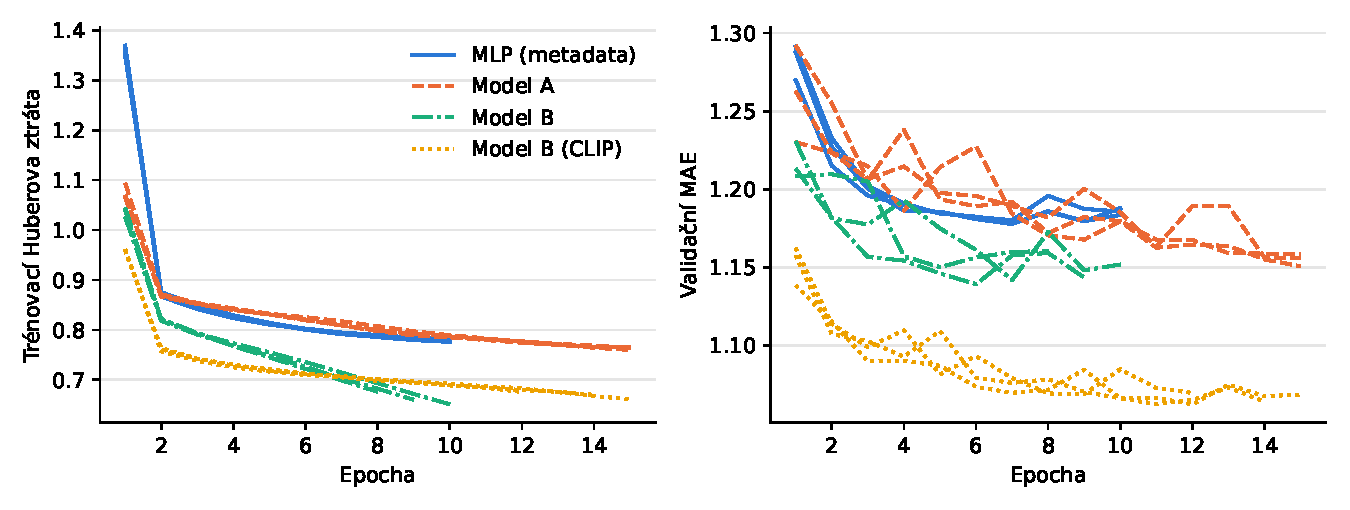
\includegraphics[width=\textwidth]{krivky.pdf}
    \caption{Trénovací Huberova ztráta (vlevo) a validační MAE (vpravo) po epochách,
    všechny tři seedy každého modelu.}
    \label{fig:krivky}
\end{figure}

U modelu B trénovací ztráta dál klesá, zatímco validační MAE se po 5. až 7. epoše přestane
zlepšovat (obrázek~\ref{fig:krivky}). Hlava se začíná přeučovat a trénování ukončí early stopping.
Validační MAE modelu A kolísá, ale klesá až do poslední epochy a nejnižší je v 15. epoše u všech
tří seedů. Model A tedy spíše nebyl dotrénován a limit počtu epoch ho mohl omezit. Model
s encoderem CLIP má nižší validační chybu než ostatní modely už od první epochy.

\begin{figure}[h]
    \centering
    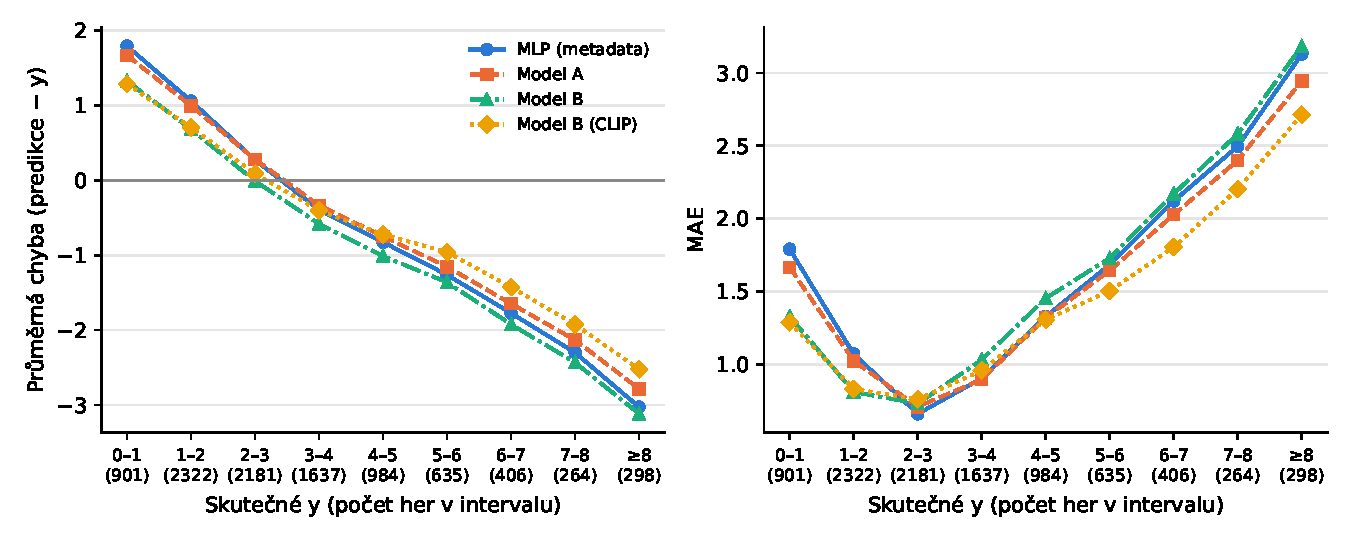
\includegraphics[width=\textwidth]{chyby.pdf}
    \caption{Průměrná chyba (predikce $-$ $y$, vlevo) a MAE (vpravo) na testovací množině podle
    skutečné hodnoty $y$. Chyba každé hry je zprůměrována přes tři seedy, v závorce je počet her
    v intervalu.}
    \label{fig:chyby}
\end{figure}

Všechny modely přeceňují hry s malým počtem recenzí a podceňují velmi populární hry
(obrázek~\ref{fig:chyby}), predikce jsou tedy stažené ke středu rozdělení. U her s $y \ge 8$ je průměrná chyba mezi $-2{,}5$ a $-3{,}1$,
skutečný počet recenzí je tedy přibližně 12- až 23krát vyšší než předpověď. Obrázky pomáhají
hlavně u málo populárních her: pro $y < 1$ je MAE nad samotnými metadaty 1,79, s modelem B 1,33
a s modelem s encoderem CLIP 1,29. Encoder CLIP jako jediný výrazněji zmenšuje podhodnocení
nejpopulárnějších her.

\subsection*{Výpočetní nároky}

\begin{table}[h]
    \centering
    \begin{tabular}{lrrrr}
        \toprule
        Model & Trénované parametry & Trénování [min] & Epocha [s] & Inference [her/s] \\
        \midrule
        MLP (metadata) & 10\,113 & 0,1 & 0,6 & 598\,152 \\
        Model A & 97\,809 & 58,4 & 233 & 1\,425 \\
        Model B & 54\,209 & 48,8 & 329 & 326 \\
        Model B (CLIP) & 37\,825 & 29,6 & 125 & 953 \\
        \bottomrule
    \end{tabular}
    \caption{Výpočetní nároky: průměr přes tři seedy, čas epochy jako medián.
    AMD Radeon RX 9070 XT (ROCm, Windows), bfloat16. Inference: dávka 128, 5 zahřívacích
    a 50 měřených průchodů, bez načítání dat.}
    \label{tab:naroky}
\end{table}

Model B má přibližně poloviční počet trénovaných parametrů než model A, každý průchod ale
počítá celý zmrazený ConvNeXt-Tiny (27,8 milionu parametrů), a jeho inference je proto přibližně
čtyřikrát pomalejší (tabulka~\ref{tab:naroky}). Celkový čas trénování modelu B je přesto kratší,
protože early stopping ho zastavil po 8 až 10 epochách. Model s encoderem CLIP
(87,9 milionu parametrů) trénoval i predikoval rychleji než model B. Čas epochy zahrnuje
načítání obrázků a validaci. Opakované měření inference se u modelu A lišilo o 27\,\%.
